\documentclass[11 pt , a 4 paper ]{article}
\usepackage[dvipsnames]{xcolor}
\usepackage{tikz}
\usetikzlibrary{shapes}
\usetikzlibrary{calc}
\usepackage{anyfontsize}
\usepackage{sectsty}
\usepackage{graphicx} % Required for inserting images
\usepackage{amsmath} % AMS Base Package
\usepackage{amssymb} % AMS Symbols
\usepackage{amsthm} % AMS
\usepackage{hyperref} % Hyperrefferings
\usepackage{amsfonts} % AMS Fonts
\usepackage{tabto}
\usepackage{enumitem}
\usepackage[utf8]{inputenc}
\usepackage{pgfplots} % Plots
\pgfplotsset{width=10cm,compat=1.9}
\usepackage[margin=1cm]{geometry}
\usepackage[skins]{tcolorbox}
\usepackage{listings}  %Code blocks
\usepackage{enumitem} % Fancy Bullet points
\usepackage{array} %Tables
\usepackage{xcolor} % Text Color
\usepackage{svg}
\usepackage{pdfpages}
\usepackage{array} %Tables
\usepackage[table]{xcolor} % Text Color
\usepackage{float}
\usepackage{booktabs} % For professional horizontal lines
\usepackage{siunitx}  % For aligning numbers on the decimal point
\usepackage[table]{xcolor} % For adding color (e.g., zebra stripes)
\usepackage{tabularx} % For tables that adjust to a specific width
\usepackage{ragged2e} % for '\RaggedRight' macro (suppress full justification)
\usepackage{booktabs} % for '\toprule', '\midrule', and '\bottomrule' macros

\definecolor{aqua}{RGB}{3,164,186}
\definecolor{grey}{RGB}{200,200,200}


{\Huge\title {CSIT123 - Computing and Cyber Security Fundamentals}}

\author{Ruhan Shafi}
\date{\today}

\theoremstyle{definition}
\newtheorem{thm}{Defination}


\usepackage{xcolor}

\definecolor{codegreen}{rgb}{0,0.6,0}
\definecolor{codegray}{rgb}{0.5,0.5,0.5}
\definecolor{codepurple}{rgb}{0.58,0,0.82}
\definecolor{backcolour}{rgb}{0.95,0.95,0.92}

\lstdefinestyle{mystyle}{
	backgroundcolor=\color{backcolour},   
	commentstyle=\color{codegreen},
	keywordstyle=\color{magenta},
	numberstyle=\tiny\color{codegray},
	stringstyle=\color{codepurple},
	basicstyle=\ttfamily\footnotesize,
	breakatwhitespace=false,         
	breaklines=true,                 
	captionpos=b,                    
	keepspaces=true,                 
	numbers=left,                    
	numbersep=5pt,                  
	showspaces=false,                
	showstringspaces=false,
	showtabs=false,                  
	tabsize=2
}

\lstset{style=mystyle}
\begin{document}
		\pagestyle{empty}
		\begin{tikzpicture}[remember picture,overlay]
				\fill[BlueViolet] (current page.south west) rectangle (current page.north east);
				\begin{scope}
						\foreach \i in {2.5,...,22}
						{\node[rounded corners,BlueViolet!90,draw,regular polygon,regular polygon sides=6, minimum size=\i cm,ultra thick] at ($(current page.west)+(2.5,-5)$) {} ;}
					\end{scope}
				\node[rounded corners,fill=BlueViolet!95,text =BlueViolet!5,regular polygon,regular polygon sides=6, minimum size=2.5 cm,inner sep=0,ultra thick] at ($(current page.west)+(2.5,-5)$) {{\includegraphics[scale=.06]{~/Notes/LaTex Work/logo4.png}}};
				\foreach \i in {0.5,...,22}		
				{\node[rounded corners,BlueViolet!90,draw,regular polygon,regular polygon sides=6, minimum size=\i cm,ultra thick] at ($(current page.north west)+(2.5,0)$) {} ;}
				\foreach \i in {0.5,...,22}
				{\node[rounded corners,BlueViolet!98,draw,regular polygon,regular polygon sides=6, minimum size=\i cm,ultra thick] at ($(current page.north east)+(0,-9.5)$) {} ;}
				\foreach \i in {12}
				{\node[fill = BlueViolet
						,rounded corners,draw=BlueViolet,regular polygon,regular polygon sides=6, minimum size=\i cm,ultra thick] at ($(current page.south east)+(-0.2,-0.45)$) {} ;}
				\foreach \i in {21,...,6}
				{\node[BlueViolet!95,rounded corners,draw,regular polygon,regular polygon sides=6, minimum size=\i cm,ultra thick] at ($(current page.south east)+(-0.2,-0.45)$) {} ;}
				\node[left,BlueViolet!5,minimum width=0.625*\paperwidth,minimum height=3cm, rounded corners] at ($(current page.north east)+(0,-9.5)$){{\fontsize{25}{30} \selectfont \bfseries Assessment 3 Lab Report}};
				\node[left,BlueViolet!10,minimum width=0.625*\paperwidth,minimum height=2cm, rounded corners] at ($(current page.north east)+(0,-11)$){{\huge \textit{Foundations of Robotics}}};
				\node[left,BlueViolet!5,minimum width=0.625*\paperwidth,minimum height=2cm, rounded corners] at ($(current page.north east)+(0,-13)$){{\Large \textsc{Ruhan Shafi}}};
			\end{tikzpicture}
	\newpage
	\ \vskip -1cm
	\rightline{\includegraphics[scale=.06]{~/Notes/LaTex Work/logo3.png}}
	
	\vskip -40pt
	
	\noindent
	{Foundations of Robotics | Ruhan Shafi (u3284342)}
	
	\vskip 5pt
	
	\noindent{\bf\Large Assessment 3: Lab Report}
	
	\vskip 7pt
	{\color{aqua}\hrule height 1pt}
	{\color{grey}\hrule height 1pt}
	
	\vskip 5pt

  \section*{Task 1}
  \subsection*{Part 1 - The Build}
  \begin{center}
    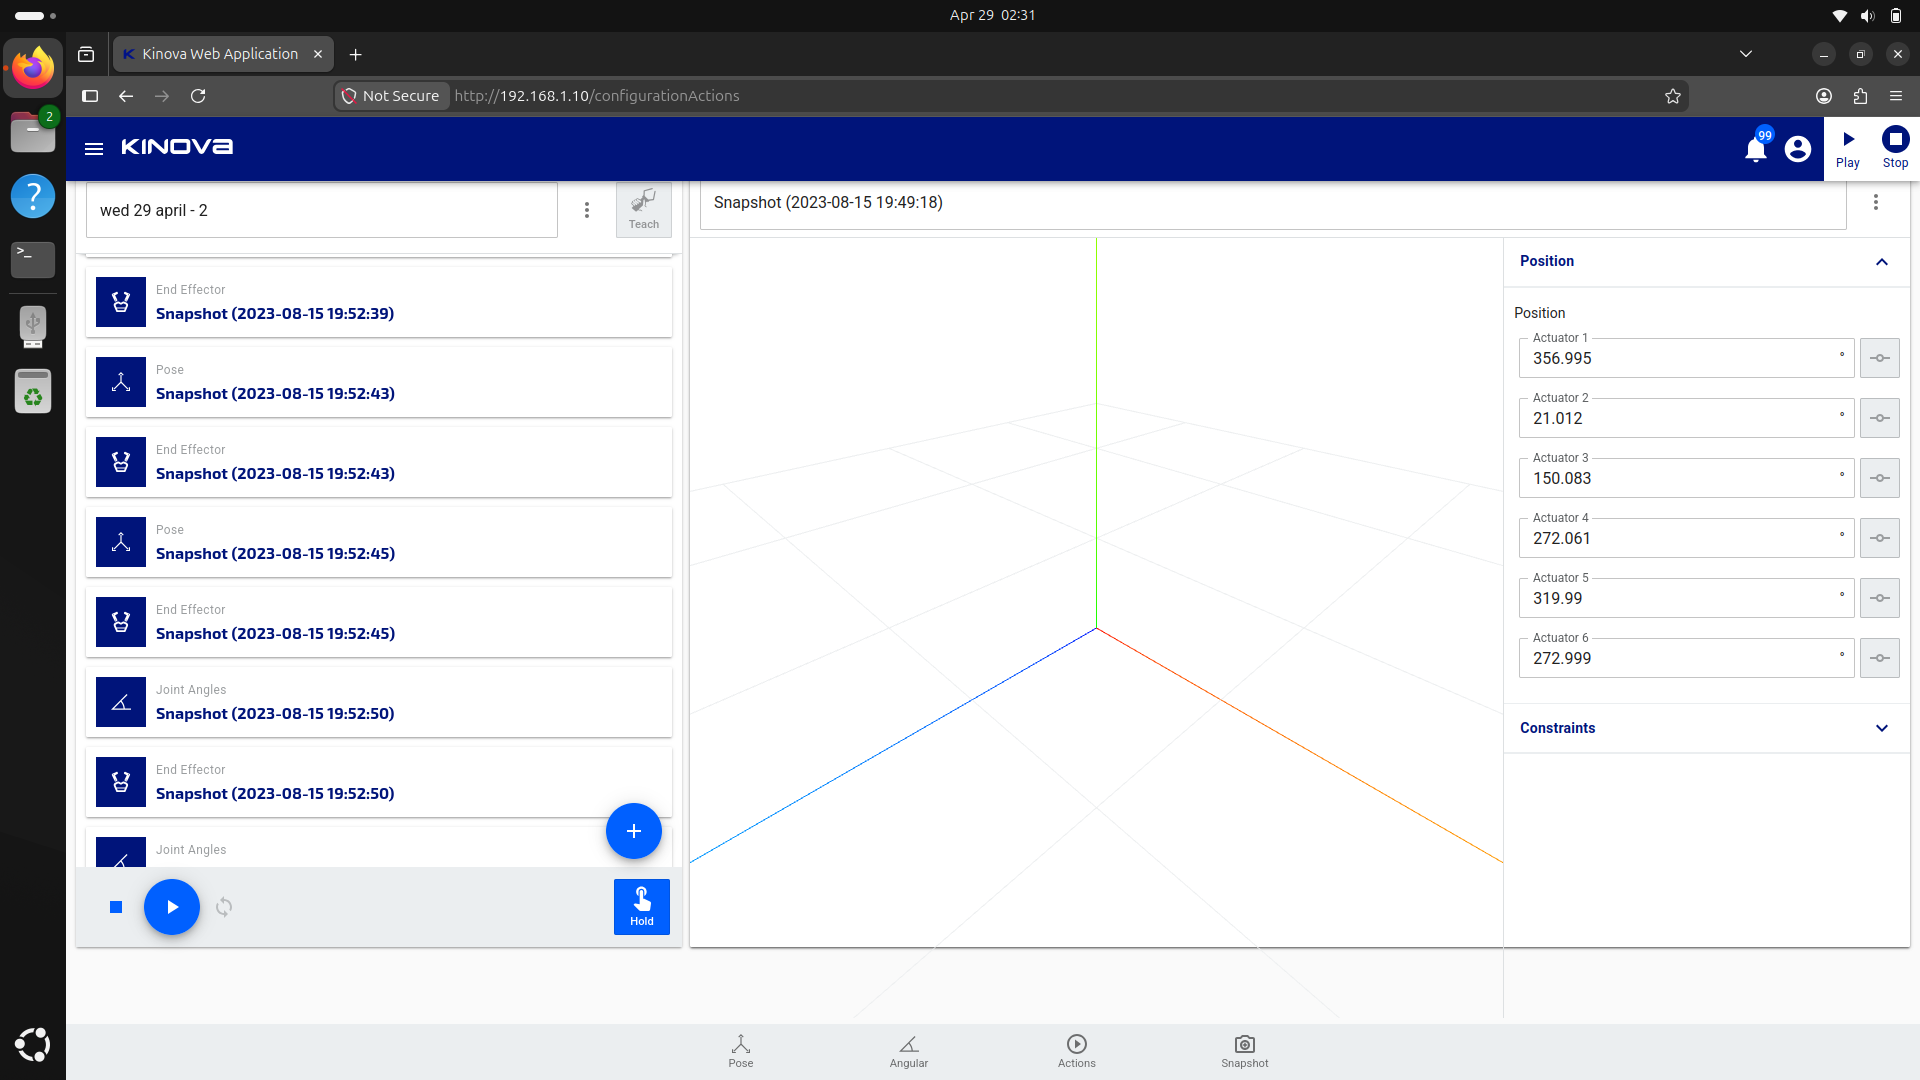
\includegraphics[width=0.8\textwidth]{A1.png}
    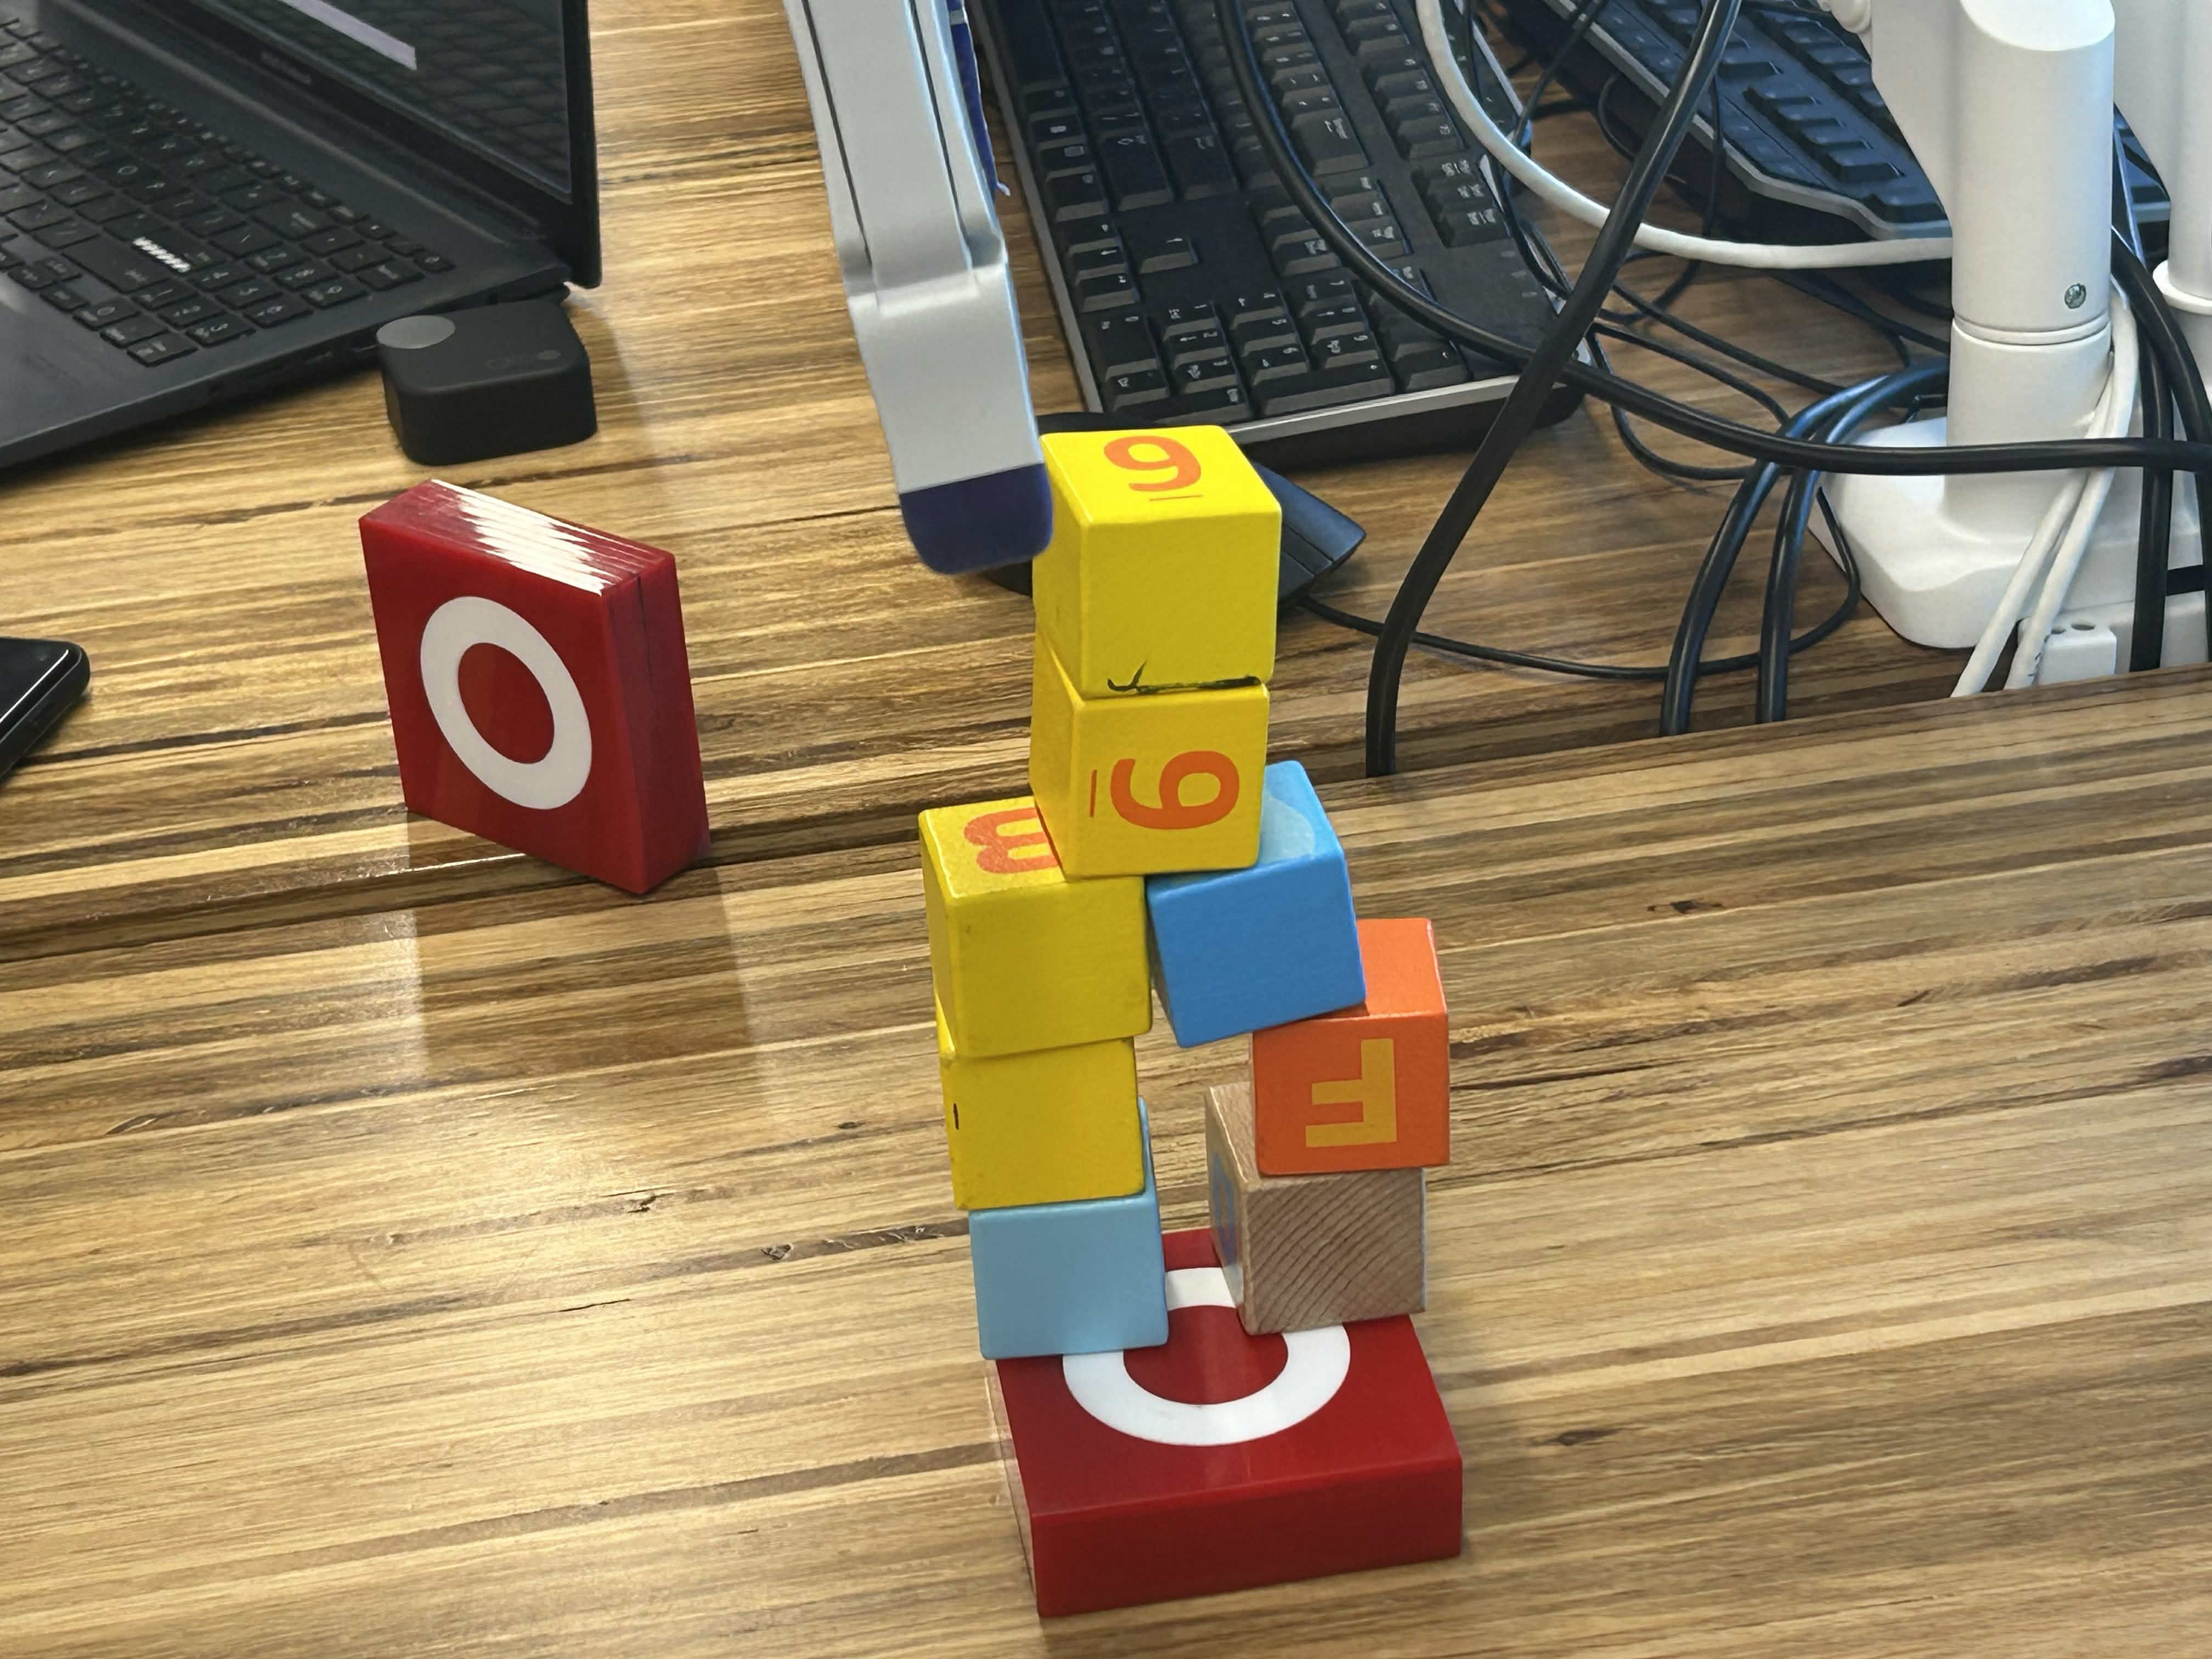
\includegraphics[width=0.8\textwidth]{A2.jpg}
  \end{center}

  \subsection*{Part B - The Simulation}

  \begin{center}
    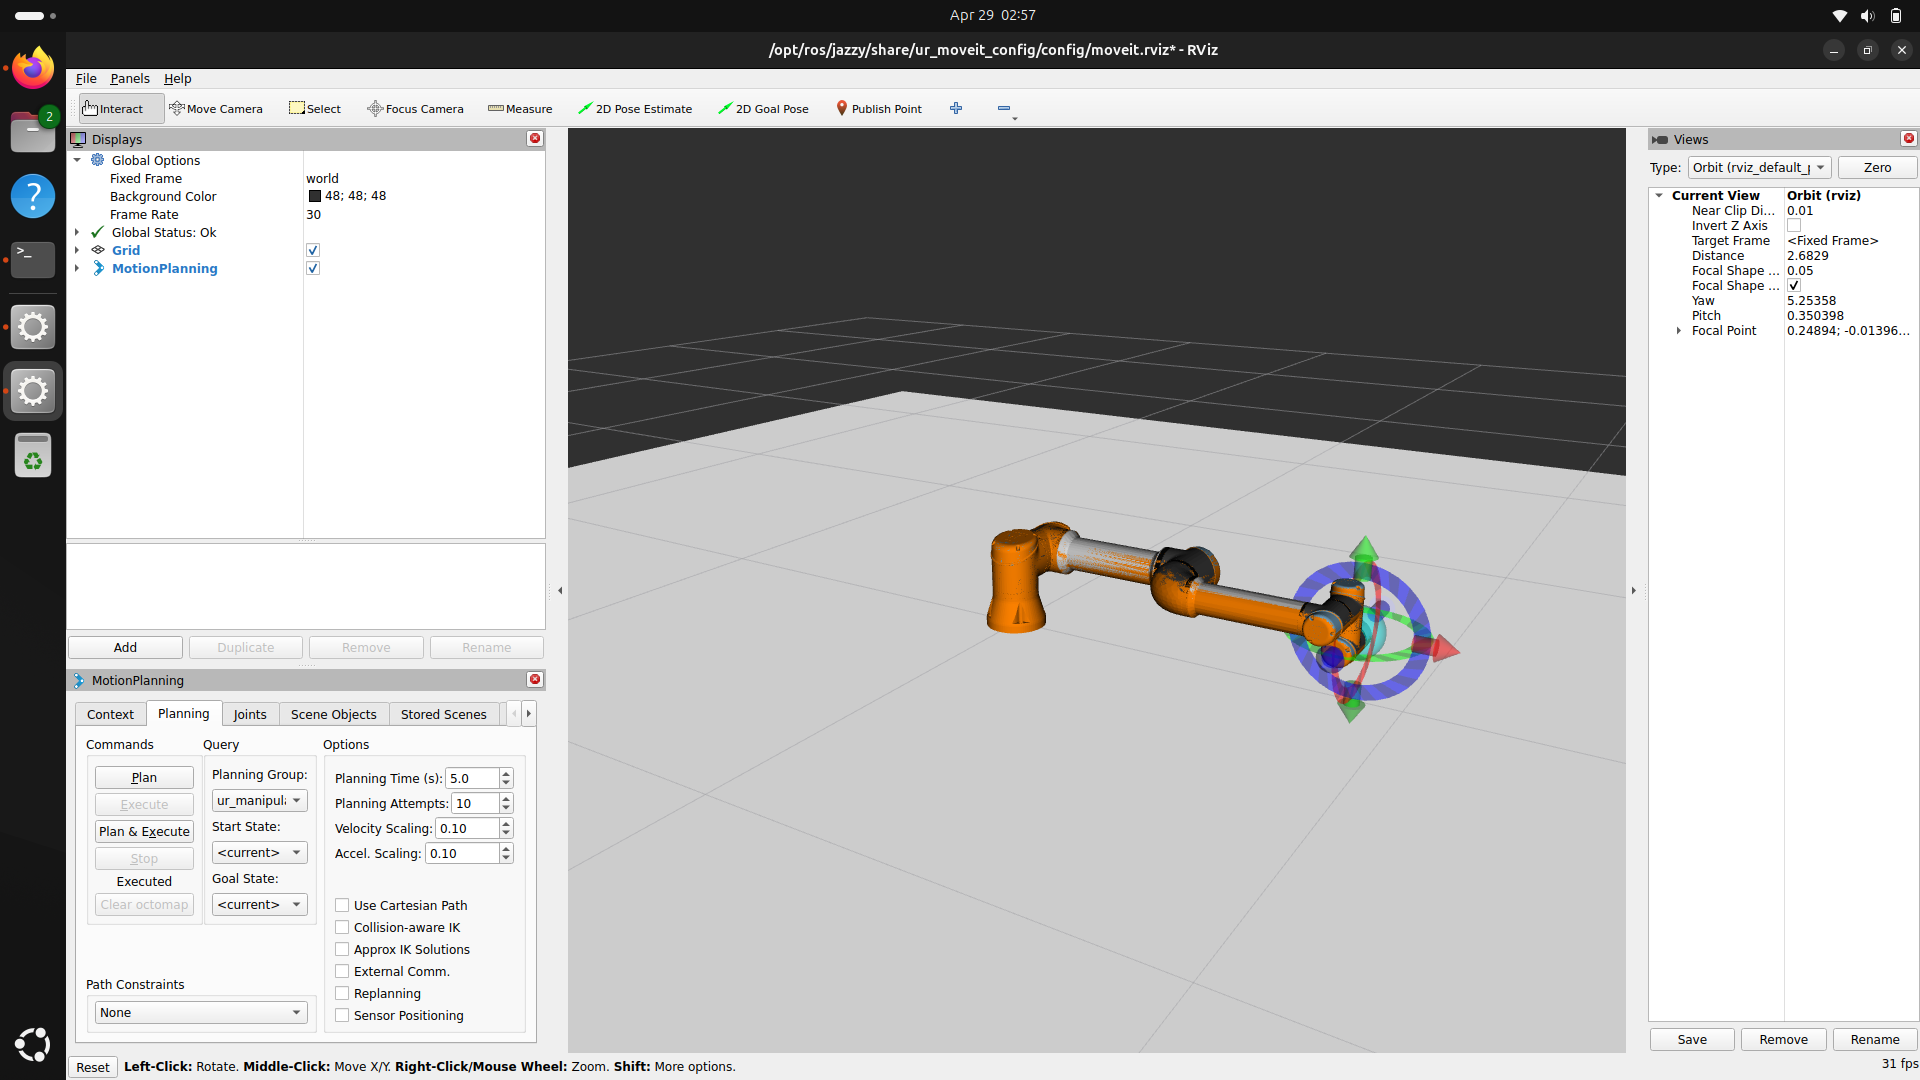
\includegraphics[width=0.8\textwidth]{1ba.png}
    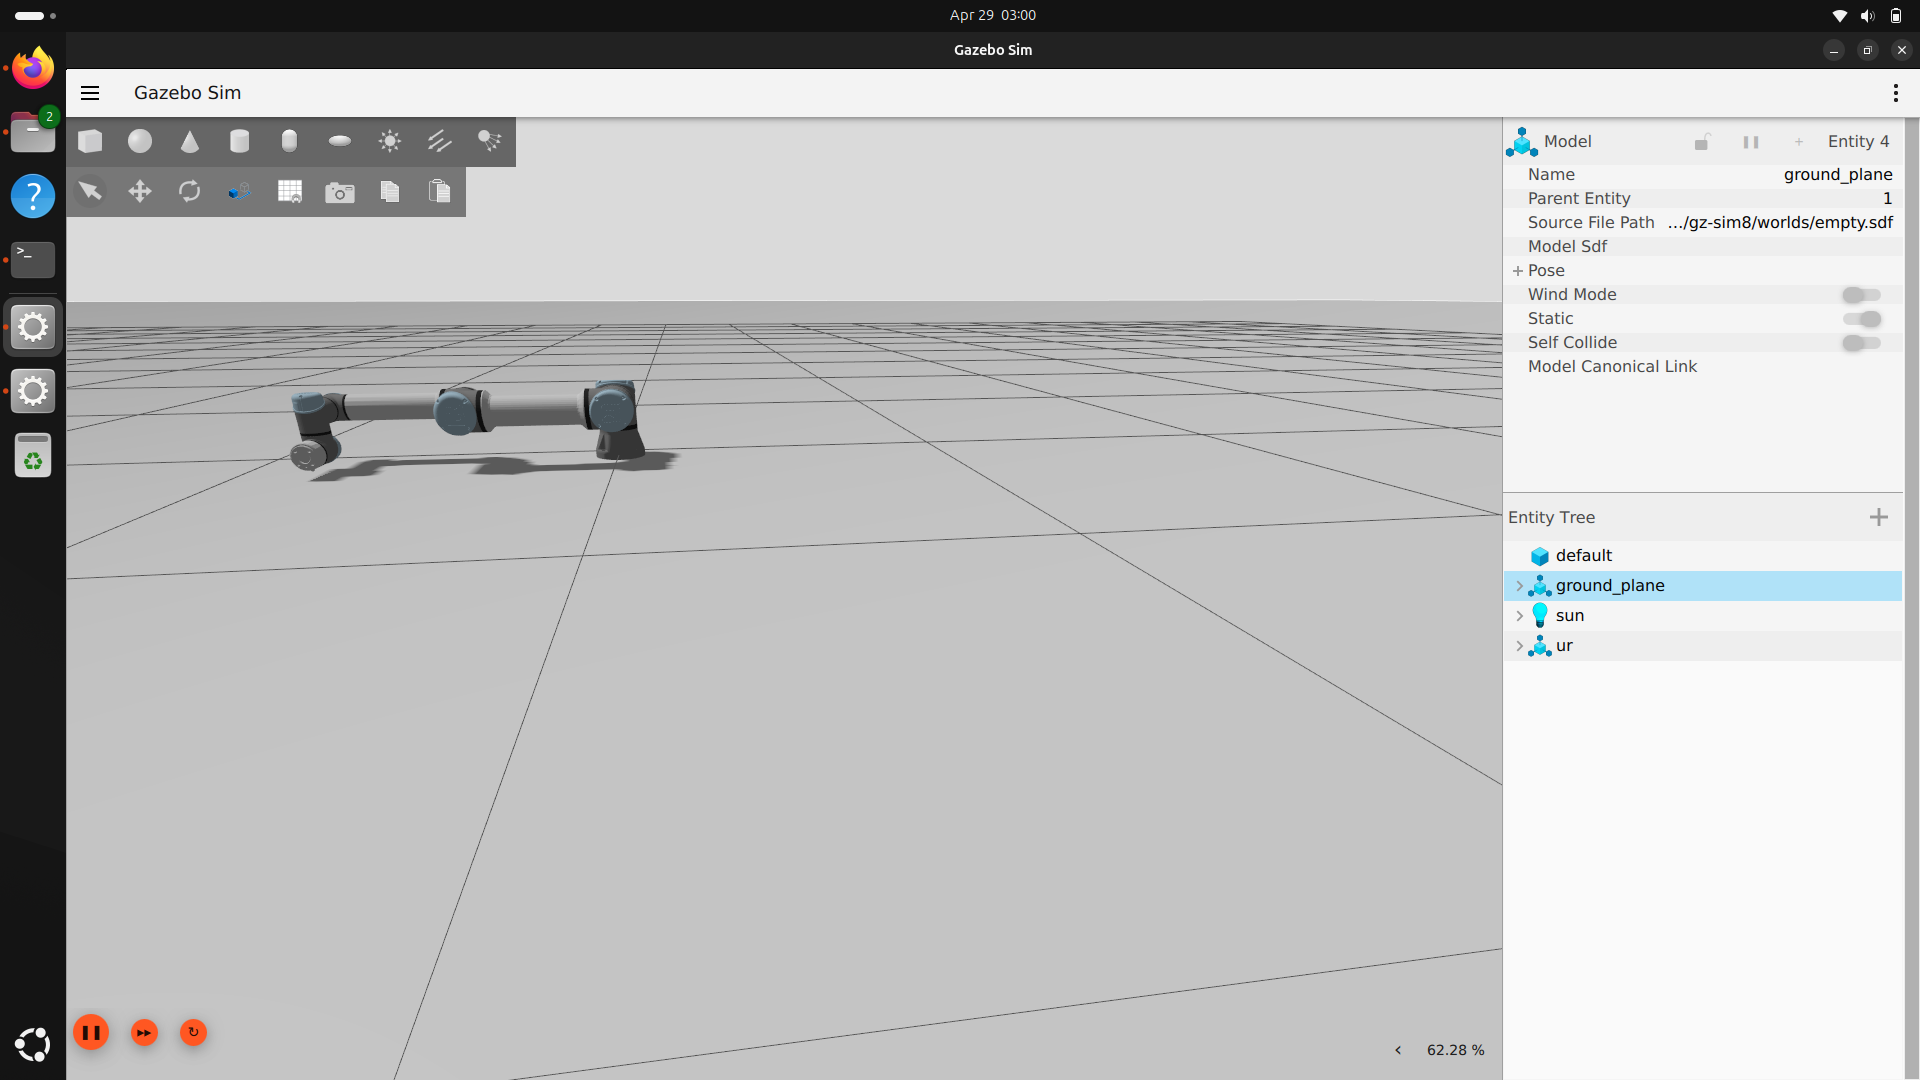
\includegraphics[width=0.8\textwidth]{1bb.png}
  \end{center}
  \section*{Task 2 - Simple Two-Link Manipulator}
  \subsection*{Part 1 - Manual Working Out}
  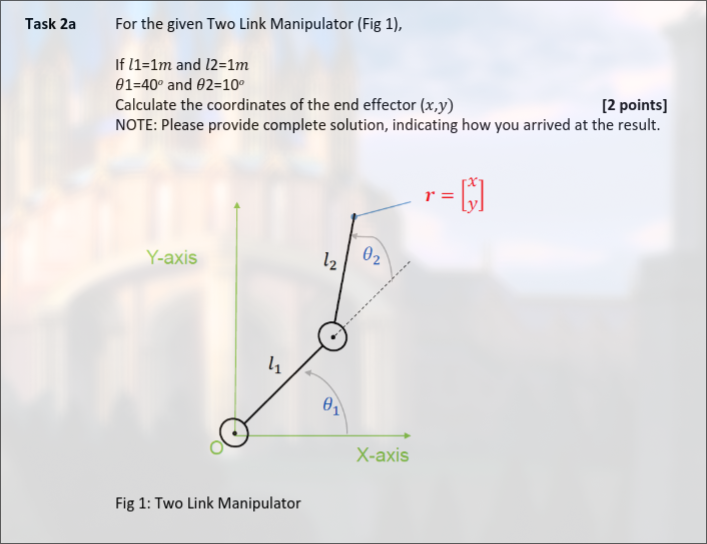
\includegraphics[width=0.8\textwidth]{task2.png}
  \newline\noindent Given the Two-Link Manipulator in Fig 1, with the following parameters:
\begin{itemize}
    \item $l_1 = 1\,\text{m}$
    \item $l_2 = 1\,\text{m}$
    \item $\theta_1 = 40^\circ$
    \item $\theta_2 = 10^\circ$
\end{itemize}

\noindent The coordinates $(x, y)$ of the end effector are determined by the sum of the link vectors. Note that the angle of the second link relative to the x-axis is $(\theta_1 + \theta_2)$.

\begin{align*}
    x &= l_1 \cos(\theta_1) + l_2 \cos(\theta_1 + \theta_2) \\
    y &= l_1 \sin(\theta_1) + l_2 \sin(\theta_1 + \theta_2)
\end{align*}

Substitute the given values into the equations:
\begin{align*}
    x &= 1 \cdot \cos(40^\circ) + 1 \cdot \cos(40^\circ + 10^\circ) \\
    x &= \cos(40^\circ) + \cos(50^\circ) \\
    x &\approx 0.7660 + 0.6428 \\
    \mathbf{x} &\approx \mathbf{1.4088\,\text{m}}
\end{align*}

\begin{align*}
    y &= 1 \cdot \sin(40^\circ) + 1 \cdot \sin(40^\circ + 10^\circ) \\
    y &= \sin(40^\circ) + \sin(50^\circ) \\
    y &\approx 0.6428 + 0.7660 \\
    \mathbf{y} &\approx \mathbf{1.4088\,\text{m}}
\end{align*}


The coordinates of the end effector $\boldsymbol{r}$ are:
\[
\boldsymbol{r} = \begin{bmatrix} x \\ y \end{bmatrix} \approx \begin{bmatrix} 1.4088 \\ 1.4088 \end{bmatrix} \,\text{m}
\]
\subsection*{Part B - Pseudo Code}
Write a suitable algorithm to calculate the Forward Kinematics of a 2-link manipulator robot with link lengths of $l_1$, $l_2$ and joint angles $\theta_{1}$, $\theta_{2}$ respectively.


\begin{lstlisting}[mathescape=true]// Forward Kinematics for a 2-Link Planar Manipulator
// Inputs:  l1, l2      - link lengths in metres
//          theta1      -  joint 1 angle in degrees (measured from X-axis)
//          theta2      - joint 2 angle in degrees (measured relative to link 1)
// Outputs: x, y        - end effector position in metres
// Constant: PI $\leftarrow$ 3.14159265

METHOD ForwardKinematics(l1, l2, theta1, theta2)

    // Step 1: Convert joint angles from degrees to radians
    theta1_rad $\leftarrow$ theta1 * (PI / 180)
    theta2_rad $\leftarrow$ theta2 * (PI / 180)

    // Step 2: Calculate the sum of joint angles
    // This gives the absolute angle of link 2 relative to the X-axis
    theta_sum $\leftarrow$ theta1_rad + theta2_rad

    // Step 3: Calculate end effector x coordinate
    // x = l1*cos(theta1) + l2*cos(theta1 + theta2)
    x $\leftarrow$ (l1 * COS(theta1_rad)) + (l2 * COS(theta_sum))

    // Step 4: Calculate end effector y coordinate
    // y = l1*sin(theta1) + l2*sin(theta1 + theta2)
    y $\leftarrow$ (l1 * SIN(theta1_rad)) + (l2 * SIN(theta_sum))

    // Step 5: Return the end effector position vector
    PRINT "End Effector Position:"
    PRINT "x = " + x
    PRINT "y = " + y

    RETURN x, y

ENDMETHOD

// --- Main Program ---

READ l1
READ l2
READ theta1
READ theta2

CALL ForwardKinematics(l1, l2, theta1, theta2) RETURNING x, y
\end{lstlisting}

\section*{Task 3 - Forward Kinematics}
\subsection*{Task 3a - Python Script}
\noindent\textbf{Screenshot of the resulting DH parameter table and graphical model of the robot configuration.}
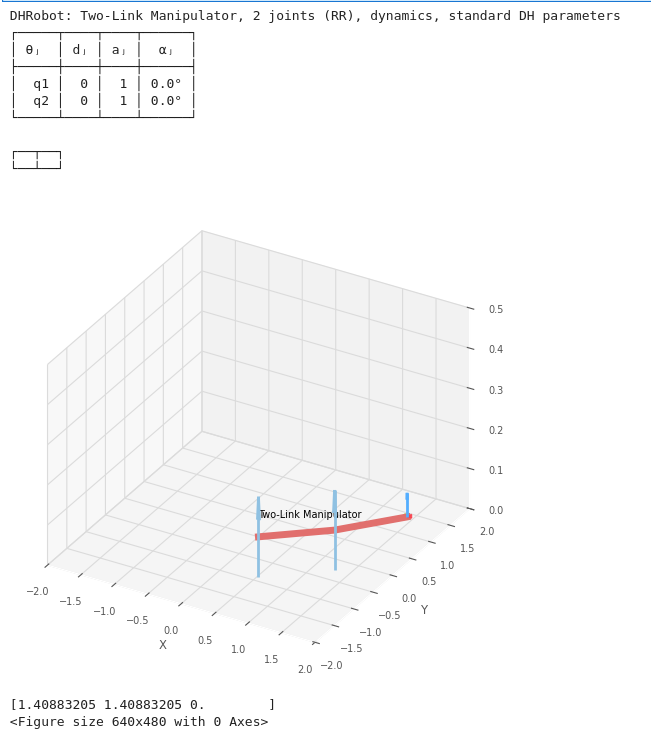
\includegraphics[width=0.65\textwidth]{task3a.png}
\newline\noindent\textbf{Record the output and compare the results to what you calculated in Task 2a}
\newline\noindent As seen in the screenshot above, the returned value is the same as the ones calculated in Task 2a, thus validating the calculations performed in that task.
\subsection*{Task 3b - DH Parameters}
\textbf{Task 1 - Draw the Link diagram}\newline
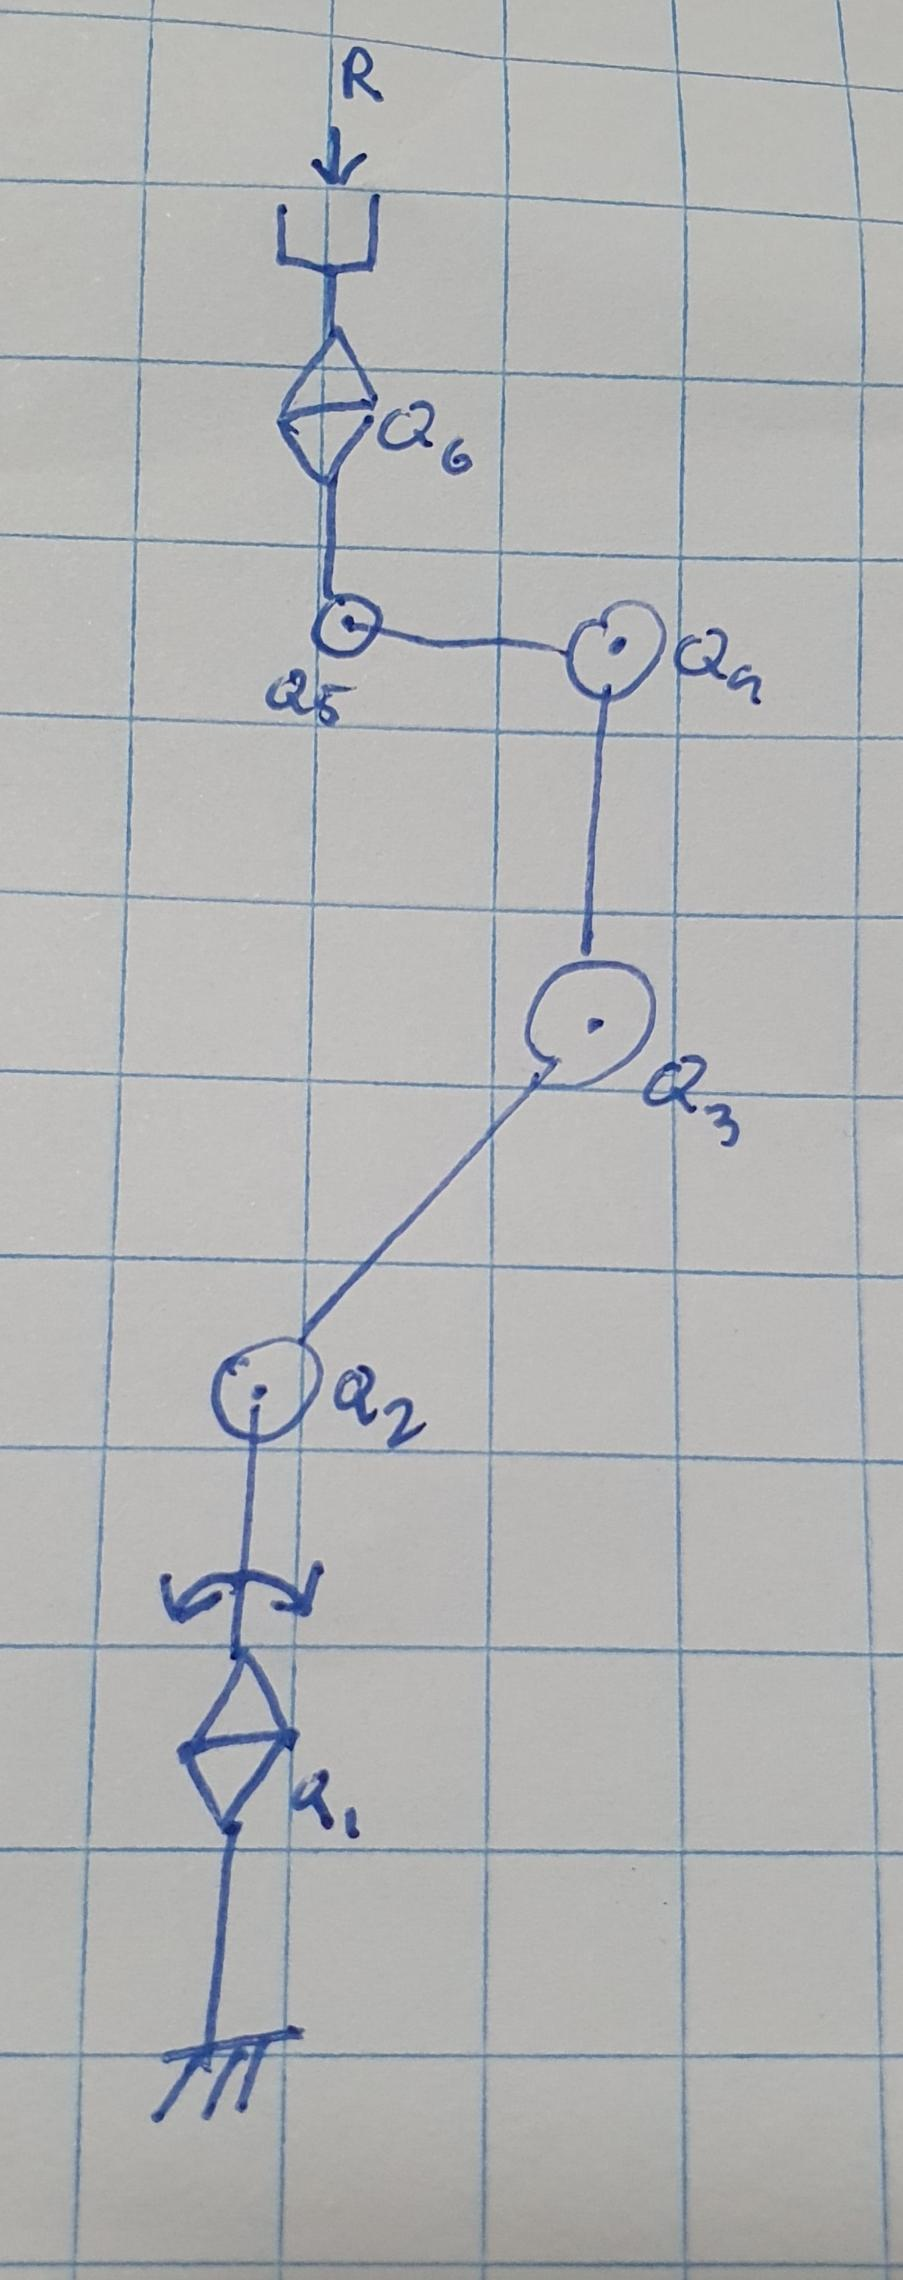
\includegraphics[scale=0.2]{link.jpg} \newline

\textbf{Task 2 - Tabulate the DH parameters}\\
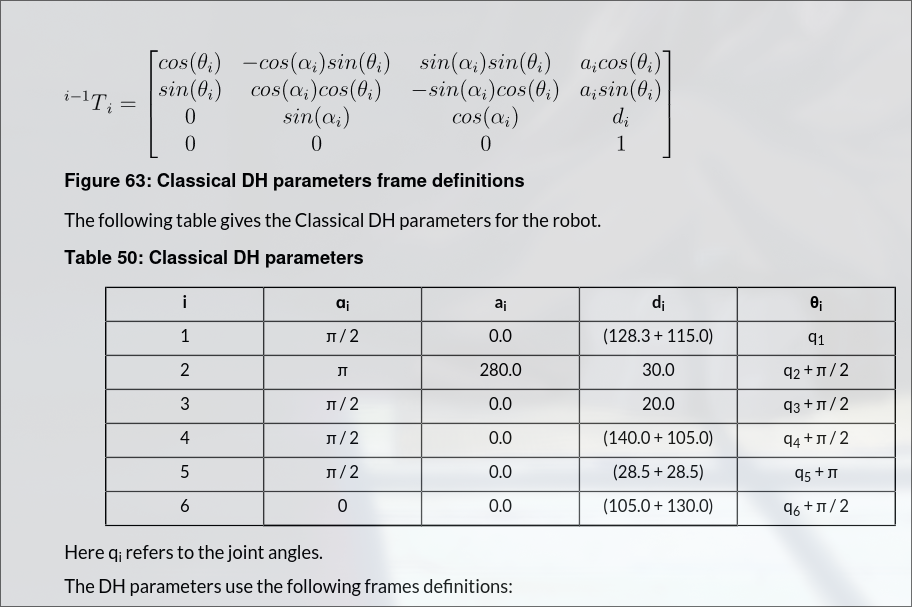
\includegraphics[width=0.8\textwidth]{3ai.png}
\begin{center}\noindent \textit{Sourced from the Official Kinova Gen3 lite robot User guide: Page 135}\end{center}
\subsection*{Task 3c- Python Script}
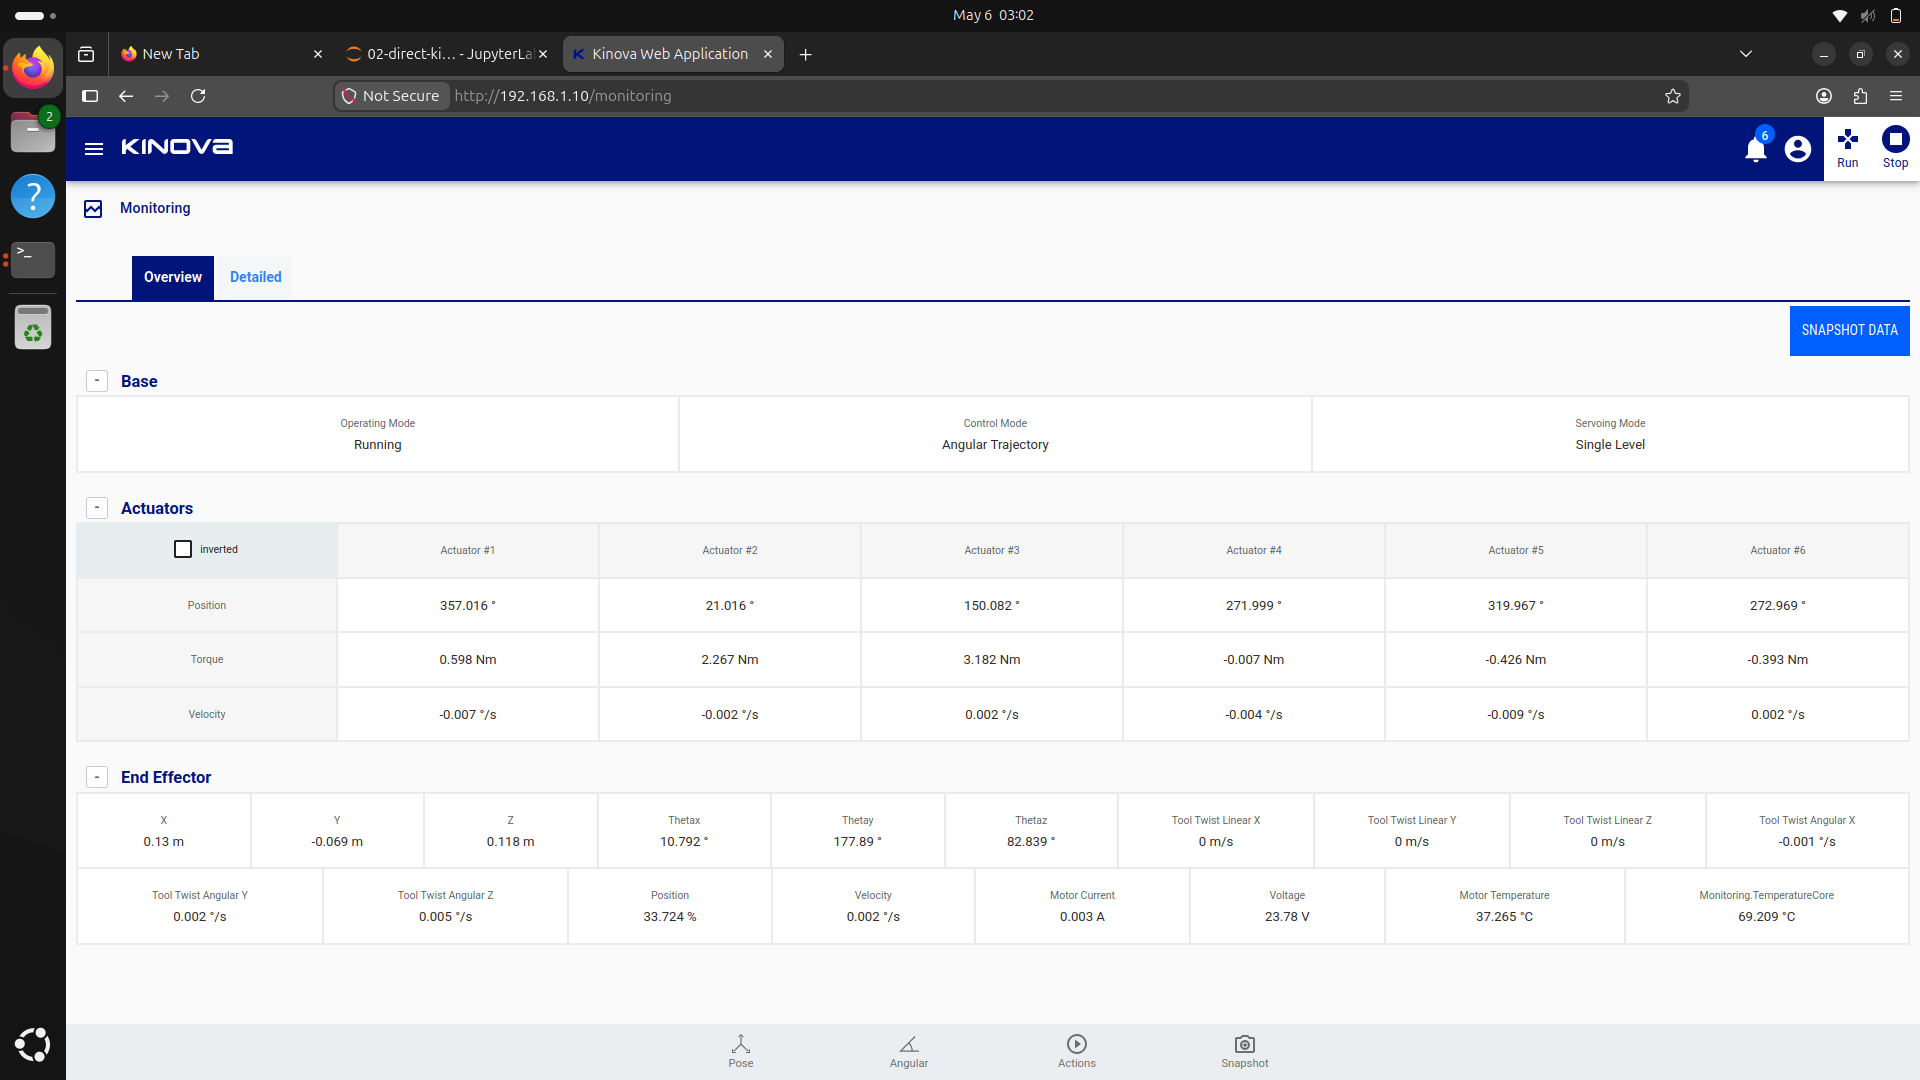
\includegraphics[width=0.8\textwidth]{Task3ci.png}
\newline\noindent\textbf{Source code to generate the Kinova robot model using the Robotics Toolbox}\\
\lstinputlisting[language=Python]{task3.py}
\noindent\textbf{Screenshot of final pose of the robot as generated by the robotics toolbox and output of the command \texttt{print(pose.t)}}
\newline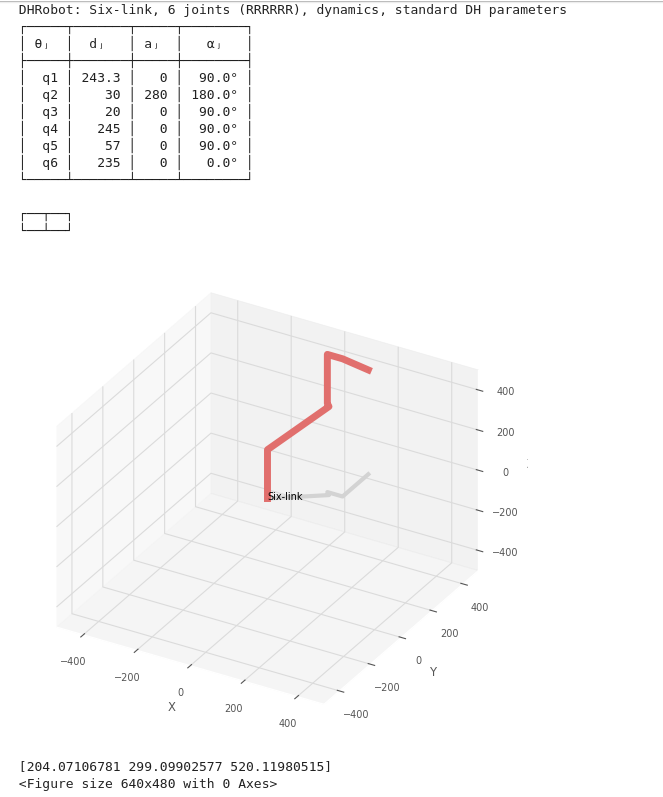
\includegraphics[width=0.8\textwidth]{task3cii.png}
\end{document}
